\documentclass[svgnames,11pt]{beamer}
\input{/home/tof/Documents/Cozy/latex-include/preambule_commun.tex}
\input{/home/tof/Documents/Cozy/latex-include/preambule_beamer.tex}
\usepackage{pgfpages} \setbeameroption{show notes on second screen=left}
\author[]{Christophe Viroulaud}
\title{Requêtes avancées}
\date{\framebox{\textbf{BDD 06}}}
%\logo{}
\institute{Terminale - NSI}

\begin{document}
\begin{frame}
\titlepage
    \note[item]{\fcolorbox{black}{red}{{\LARGE toujours sur bd-avec-emprunts.db 
    }}}
     \note[item]{\fcolorbox{black}{red}{{\LARGE (version initiale: )}}}
         \note[item]{\fcolorbox{black}{red}{{\LARGE y a eu des modif dans cours précédent}}}
\end{frame}
\begin{frame}[fragile]
    \frametitle{}

\begin{center}
\begin{lstlisting}[language=SQL , basicstyle=\ttfamily\small, xleftmargin=1em, xrightmargin=0em]
INSERT INTO Animaux (nom, age, id_espece) VALUES 
("Minou", 15, 2);
\end{lstlisting}
\captionof{code}{Une requête peu pratique}
\label{CODE}
\end{center}
\note{Il faut connaître l'id de l'espèce}
\end{frame}
\begin{frame}
    \frametitle{}

    \begin{framed}
        \centering Comment mettre en relation plusieurs tables?
    \end{framed}

\end{frame}
\section{Fonctions d'agrégation}
\begin{frame}[fragile]
    \frametitle{Fonctions d'agrégation}

    Ce sont des fonctions qui vont regrouper les lignes. La plupart des fonctions d'agrégation vont permettre de faire des statistiques sur les données. 
\begin{center}
\begin{lstlisting}[language=SQL , basicstyle=\ttfamily\small, xleftmargin=1em, xrightmargin=0em]
SELECT COUNT(*) FROM Bandes_dessinees WHERE 
serie = "Aya de Yopougon";
\end{lstlisting}
\captionof{code}{\centering Compte le nombre de lignes (donc d'albums) de la série \emph{Aya de Yopougon}}
\label{count}
\end{center}    

\end{frame}
\begin{frame}[fragile]

\begin{aretenir}[Remarque]
Le code suivant donnerait le même résultat que le code \ref{count}.
\begin{lstlisting}[language=SQL , basicstyle=\ttfamily\small, xleftmargin=1em, xrightmargin=0em]
SELECT COUNT(titre) FROM Bandes_dessinees WHERE 
serie = "Aya de Yopougon";
\end{lstlisting}
Cependant si certaines lignes avaient un titre \textbf{\texttt{NULL}} elles ne seraient ici pas comptées.
\end{aretenir} 

\end{frame}
\begin{frame}
    \frametitle{}

    Il existe de nombreuses fonctions d'agrégation. Citons la moyenne (\texttt{\textbf{AVG}}), la somme (\texttt{\textbf{SUM}}), le maximum (\texttt{\textbf{MAX}}). La documentation en ligne détaillera de manière exhaustive ces fonctions.

\end{frame}
\begin{frame}[fragile]
    \frametitle{}

\begin{activite}
\begin{enumerate}
\item Tester la requête \ref{count}.
\item Compter le nombre total de bandes dessinées.
\item Tester la requête \ref{distinct}. Que renvoie-t-elle?
\begin{center}
\begin{lstlisting}[language=SQL , basicstyle=\ttfamily\small, xleftmargin=1em, xrightmargin=0em]
SELECT COUNT(DISTINCT id_dessinateur) FROM Bandes_dessinees;
\end{lstlisting}
\captionof{code}{Mot clé \texttt{\textbf{DISTINCT}}}
\label{distinct}
\end{center}
\end{enumerate}
\end{activite}

\end{frame}
\section{Mettre des tables en relation}
\subsection{Sous-requêtes}
\begin{frame}[fragile]
    \frametitle{Sous-requêtes}

\begin{center}
\begin{lstlisting}[language=SQL , basicstyle=\ttfamily\small, xleftmargin=1em, xrightmargin=0em]
SELECT titre FROM Bandes_dessinees WHERE id_genre = 13;
\end{lstlisting}
\captionof{code}{\centering Sélectionner toutes les bandes dessinées du genre \texttt{\textbf{jeunesse}}}
\label{jeunesse}
\end{center}   
\begin{aretenir}[Remarque]
    Il est nécessaire de connaître l'\textbf{\texttt{id}} du genre \textbf{\texttt{jeunesse}} dans la table \texttt{\textbf{Genres}}.
\end{aretenir}
\end{frame}
\begin{frame}[fragile]

\begin{center}
\begin{lstlisting}[language=SQL , basicstyle=\ttfamily\small, xleftmargin=1em, xrightmargin=0em]
SELECT id FROM Genres WHERE genre = "Jeunesse";
\end{lstlisting}
\captionof{code}{\centering Sélectionner l'\textbf{\texttt{id}} du genre \texttt{\textbf{jeunesse}}}
\end{center}   

\end{frame}
\begin{frame}[fragile]

\begin{center}
\begin{lstlisting}[language=SQL , basicstyle=\ttfamily\small, xleftmargin=1em, xrightmargin=0em]
SELECT titre FROM Bandes_dessinees 
    WHERE id_genre = (SELECT id FROM Genres WHERE genre = "Jeunesse");
\end{lstlisting}
\captionof{code}{\centering Combiner les requêtes}
\label{sous}
\end{center}   
    
    \end{frame}
\begin{frame}[fragile]
    \frametitle{}

\begin{activite}
\begin{enumerate}
\item Tester la requête \ref{sous}.
\item Sélectionner les titres de livres dessinés par Joann Sfar.
\item Compter les titres publiés par l'éditeur Delcourt.
\item Que renvoie la requête \ref{isbn}?
\begin{center}
\begin{lstlisting}[language=SQL , basicstyle=\ttfamily\small, xleftmargin=1em, xrightmargin=0em]
SELECT titre FROM Bandes_dessinees WHERE 
    isbn IN (SELECT isbn FROM Emprunts WHERE id_emprunteurs = 1);
\end{lstlisting}
\captionof{code}{Sous requête}
\label{isbn}
\end{center}
\end{enumerate}
\end{activite}

\end{frame}
\begin{frame}[fragile]
\frametitle{Correction}
\begin{center}
\begin{lstlisting}[language=SQL , basicstyle=\ttfamily\small, xleftmargin=1em, xrightmargin=0em]
SELECT titre FROM Bandes_dessinees
    WHERE id_dessinateur = 
        (SELECT id FROM Auteurs
            WHERE nom = "Sfar" and
                prenom = "Joann");
\end{lstlisting}
\captionof{code}{\centering Sélectionner les titres de Joann Sfar}
\end{center}   

\end{frame}
\begin{frame}[fragile]
\begin{center}
\begin{lstlisting}[language=SQL , basicstyle=\ttfamily\small, xleftmargin=1em, xrightmargin=0em]
SELECT COUNT(titre) FROM Bandes_dessinees
    WHERE id_editeur = 
        (SELECT id FROM Editeurs
            WHERE editeur = "Delcourt");
\end{lstlisting}
\captionof{code}{\centering Compter les titres d'éditeur Delcourt}
\end{center}   

\end{frame}
\begin{frame}[fragile]
    \frametitle{}

\begin{center}
\begin{lstlisting}[language=SQL , basicstyle=\ttfamily\small, xleftmargin=1em, xrightmargin=0em]
SELECT titre FROM Bandes_dessinees WHERE 
    isbn IN (SELECT isbn FROM Emprunts WHERE id_emprunteurs = 1);
\end{lstlisting}
\captionof{code}{Sous requête}
\end{center}   
 La requête renvoie les titres empruntés par l'emprunteur 1. La clause \textbf{\texttt{IN}} peut être comparée au mot-clef \textbf{\texttt{in}} en Python.
\end{frame}
\subsection{Jointures}
\begin{frame}
    \frametitle{Jointures}

    Il existe des informations communes entre certaines tables. Une jointure permet de mettre en relation ces données (figure \ref{jointure}).
    \begin{center}
    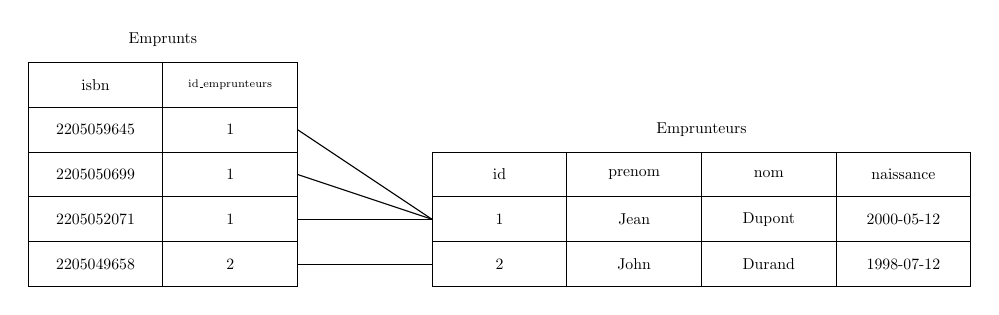
\begin{tikzpicture}[scale=0.57, transform shape]
    \node at (3,5.5) {Emprunts};
    \draw (0,0) grid[xstep=3] (6,5);
    \node at (1.5,4.5) {isbn};
    \node at (4.5,4.5) {\scriptsize id\_emprunteurs};
    
    \node at (1.5,3.5) {2205059645};
    \node at (1.5,1.5) {2205052071};
    \node at (1.5,2.5) {2205050699};
    \node at (1.5,0.5) {2205049658};
    \node at (4.5,0.5) {2};
    \node at (4.5,2.5) {1};
    \node at (4.5,1.5) {1};
    \node at (4.5,3.5) {1};
    
    \node at (15,3.5) {Emprunteurs};
    
    \draw (9,0) grid[xstep=3] (21,3);
    \node at (10.5,2.5) {id};
    \node at (13.5,2.5) {prenom};
    \node at (16.5,2.5) {nom};
    \node at (19.5,2.5) {naissance};
    
    \node at (10.5,1.5) {1};
    \node at (10.5,0.5) {2};
    \node at (13.5,1.5) {Jean};
    \node at (13.5,0.5) {John};
    \node at (16.5,1.5) {Dupont};
    \node at (16.5,0.5) {Durand};
    \node at (19.5,1.5) {2000-05-12};
    \node at (19.5,0.5) {1998-07-12};
    
    \draw (6,3.5) --(9,1.5);
    \draw (6,2.5) --(9,1.5);
    \draw (6,1.5) --(9,1.5);
    \draw (6,0.5) --(9,0.5);
    
    \end{tikzpicture}
    \captionof{figure}{Jointure des tables \emph{Emprunts} et \emph{Emprunteurs}}
    \label{jointure}
    \end{center}    

\end{frame}
\begin{frame}
    \frametitle{}

    La jointure crée un \emph{table temporaire} qui contient l'ensemble des données (figure \ref{virtuelle}).
    \begin{center}
    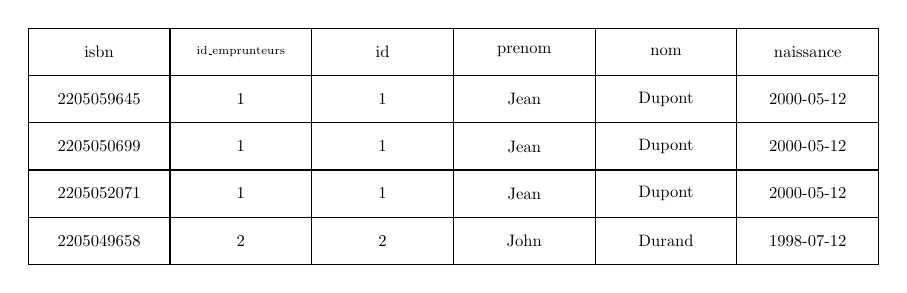
\begin{tikzpicture}[scale=0.6, transform shape]
    \draw (0,0) grid[xstep=3] (18,5);
    \node at (1.5,4.5) {isbn};
    \node at (4.5,4.5) {\scriptsize id\_emprunteurs};
    \node at (7.5,4.5) {id};
    \node at (10.5,4.5) {prenom};
    \node at (13.5,4.5) {nom};
    \node at (16.5,4.5) {naissance};
    
    \node at (1.5,3.5) {2205059645};
    \node at (1.5,1.5) {2205052071};
    \node at (1.5,2.5) {2205050699};
    \node at (1.5,0.5) {2205049658};
    
    \node at (4.5,0.5) {2};
    \node at (4.5,2.5) {1};
    \node at (4.5,1.5) {1};
    \node at (4.5,3.5) {1};
    
    \node at (7.5,3.5) {1};
    \node at (7.5,2.5) {1};
    \node at (7.5,1.5) {1};
    \node at (7.5,0.5) {2};
    
    \node at (10.5,3.5) {Jean};
    \node at (10.5,2.5) {Jean};
    \node at (10.5,1.5) {Jean};
    \node at (10.5,0.5) {John};
    
    \node at (13.5,3.5) {Dupont};
    \node at (13.5,2.5) {Dupont};
    \node at (13.5,1.5) {Dupont};
    \node at (13.5,0.5) {Durand};
    
    \node at (16.5,3.5) {2000-05-12};
    \node at (16.5,2.5) {2000-05-12};
    \node at (16.5,1.5) {2000-05-12};
    \node at (16.5,0.5) {1998-07-12};
    
    \end{tikzpicture}
    \captionof{figure}{Jointure des tables \emph{Emprunts} et \emph{Emprunteurs}}
    \label{virtuelle}
    \end{center}

\end{frame}
\begin{frame}[fragile]
    \frametitle{}
Il est alors possible de récupérer n'importe quelle information.
\begin{center}
\begin{lstlisting}[language=SQL , basicstyle=\ttfamily\small, xleftmargin=1em, xrightmargin=0em]
SELECT Emprunteurs.nom, Emprunts.isbn FROM Emprunts
JOIN Emprunteurs 
    ON Emprunts.id_emprunteurs = Emprunteurs.id;
\end{lstlisting}
\captionof{code}{\centering Renvoyer le nom des emprunteurs associés aux ISBN des bandes dessinées empruntées}
\label{jointurereq}
\end{center}
\begin{aretenir}[Remarque]
    Certaines tables peuvent avoir des attributs qui possèdent le même nom. Pour éviter les ambiguïtés, il est judicieux de nommer les attributs ainsi: \texttt{\textbf{table.attribut}}.
    \end{aretenir}

\end{frame}
\begin{frame}[fragile]
    \frametitle{}

\begin{activite}
\begin{enumerate}
\item Tester la requête \ref{jointurereq}.
\item Modifier la requête \ref{jointurereq} pour ne renvoyer que les ISBN empruntés par Dupont.
\item Il est possible d'effectuer une jointure avec plus de deux tables. Modifier la requête précédente pour renvoyer le \emph{titre} des bandes dessinées empruntées par Dupont.
\end{enumerate}
\end{activite}

\end{frame}
\begin{frame}[fragile]
    \frametitle{Correction}
\begin{center}
\begin{lstlisting}[language=SQL , basicstyle=\ttfamily\small, xleftmargin=1em, xrightmargin=0em]
SELECT Emprunteurs.nom, Emprunts.isbn FROM Emprunts
JOIN Emprunteurs 
    ON Emprunts.id_emprunteurs = Emprunteurs.id
WHERE Emprunteurs.nom = "Dupont";
\end{lstlisting}
\captionof{code}{\centering Renvoyer les bandes dessinées empruntées par Dupont}
\end{center}

\end{frame}
\begin{frame}[fragile]
    \frametitle{Correction}
\begin{center}
\begin{lstlisting}[language=SQL , basicstyle=\ttfamily\small, xleftmargin=1em, xrightmargin=0em]
SELECT Emprunteurs.nom, Emprunts.isbn FROM Emprunts
JOIN Emprunteurs 
    ON Emprunts.id_emprunteurs = Emprunteurs.id
WHERE Emprunteurs.nom = "Dupont";
\end{lstlisting}
\captionof{code}{\centering Renvoyer les isbn des bandes dessinées empruntées par Dupont}
\end{center}

\end{frame}

\begin{frame}[fragile]
    \frametitle{Correction}
\begin{center}
\begin{lstlisting}[language=SQL , basicstyle=\ttfamily\small, xleftmargin=1em, xrightmargin=0em]
SELECT Bandes_dessinees.titre FROM Bandes_dessinees
JOIN Emprunts
    ON Bandes_dessinees.isbn = Emprunts.isbn
JOIN Emprunteurs 
    ON Emprunts.id_emprunteurs = Emprunteurs.id
WHERE Emprunteurs.nom = "Dupont";
\end{lstlisting}
\captionof{code}{\centering Renvoyer les titres des bandes dessinées empruntées par Dupont}
\end{center}

\end{frame}
\begin{frame}[fragile]
    \frametitle{}

\begin{activite}
Le mot clé \emph{ORDER BY} permet de classer les résultats selon le critère donné (requête \ref{order}). Classer les résultats de la requête précédente par ordre de titre.
\begin{center}
\begin{lstlisting}[language=SQL , basicstyle=\ttfamily\small, xleftmargin=1em, xrightmargin=0em]
SELECT editeur FROM Editeurs 
WHERE editeur LIKE "G%"
ORDER BY editeur;
\end{lstlisting}
\captionof{code}{Classement des éditeurs commençant par G}
\label{order}
\end{center}
\end{activite}

\end{frame}
\begin{frame}[fragile]
    \frametitle{Correction}
\begin{center}
\begin{lstlisting}[language=SQL , basicstyle=\ttfamily\small, xleftmargin=1em, xrightmargin=0em]
SELECT Bandes_dessinees.titre FROM Bandes_dessinees
JOIN Emprunts
    ON Bandes_dessinees.isbn = Emprunts.isbn
JOIN Emprunteurs 
    ON Emprunts.id_emprunteurs = Emprunteurs.id
WHERE Emprunteurs.nom = "Dupont"
ORDER BY Bandes_dessinees.titre;
\end{lstlisting}
\captionof{code}{\centering Renvoyer les titres ordonnés.}
\end{center}

\end{frame}
\end{document}